\documentclass[12pt,a4paper]{article}
\raggedbottom

\usepackage{ugmath}
\usepackage{float}
\usepackage{placeins}
\usepackage[labelfont=bf,labelsep=space]{caption}
\usepackage{pdfpages}
\usepackage{tikz-cd}
\usepackage{amsthm}
\renewcommand{\Tr}{\operatorname{Tr}}
\newcommand{\llaves}[1]{\{#1\}}
\newcommand{\parentesis}[1]{\left(#1\right)}
\newcommand{\corchetes}[1]{\left[#1\right]}
\newcommand{\llavesgrande}[1]{\big\{#1\big\}}
\newcommand{\llavesgrandes}[1]{\left\{#1\right\}}


\begin{document}

    \thispagestyle{empty}
    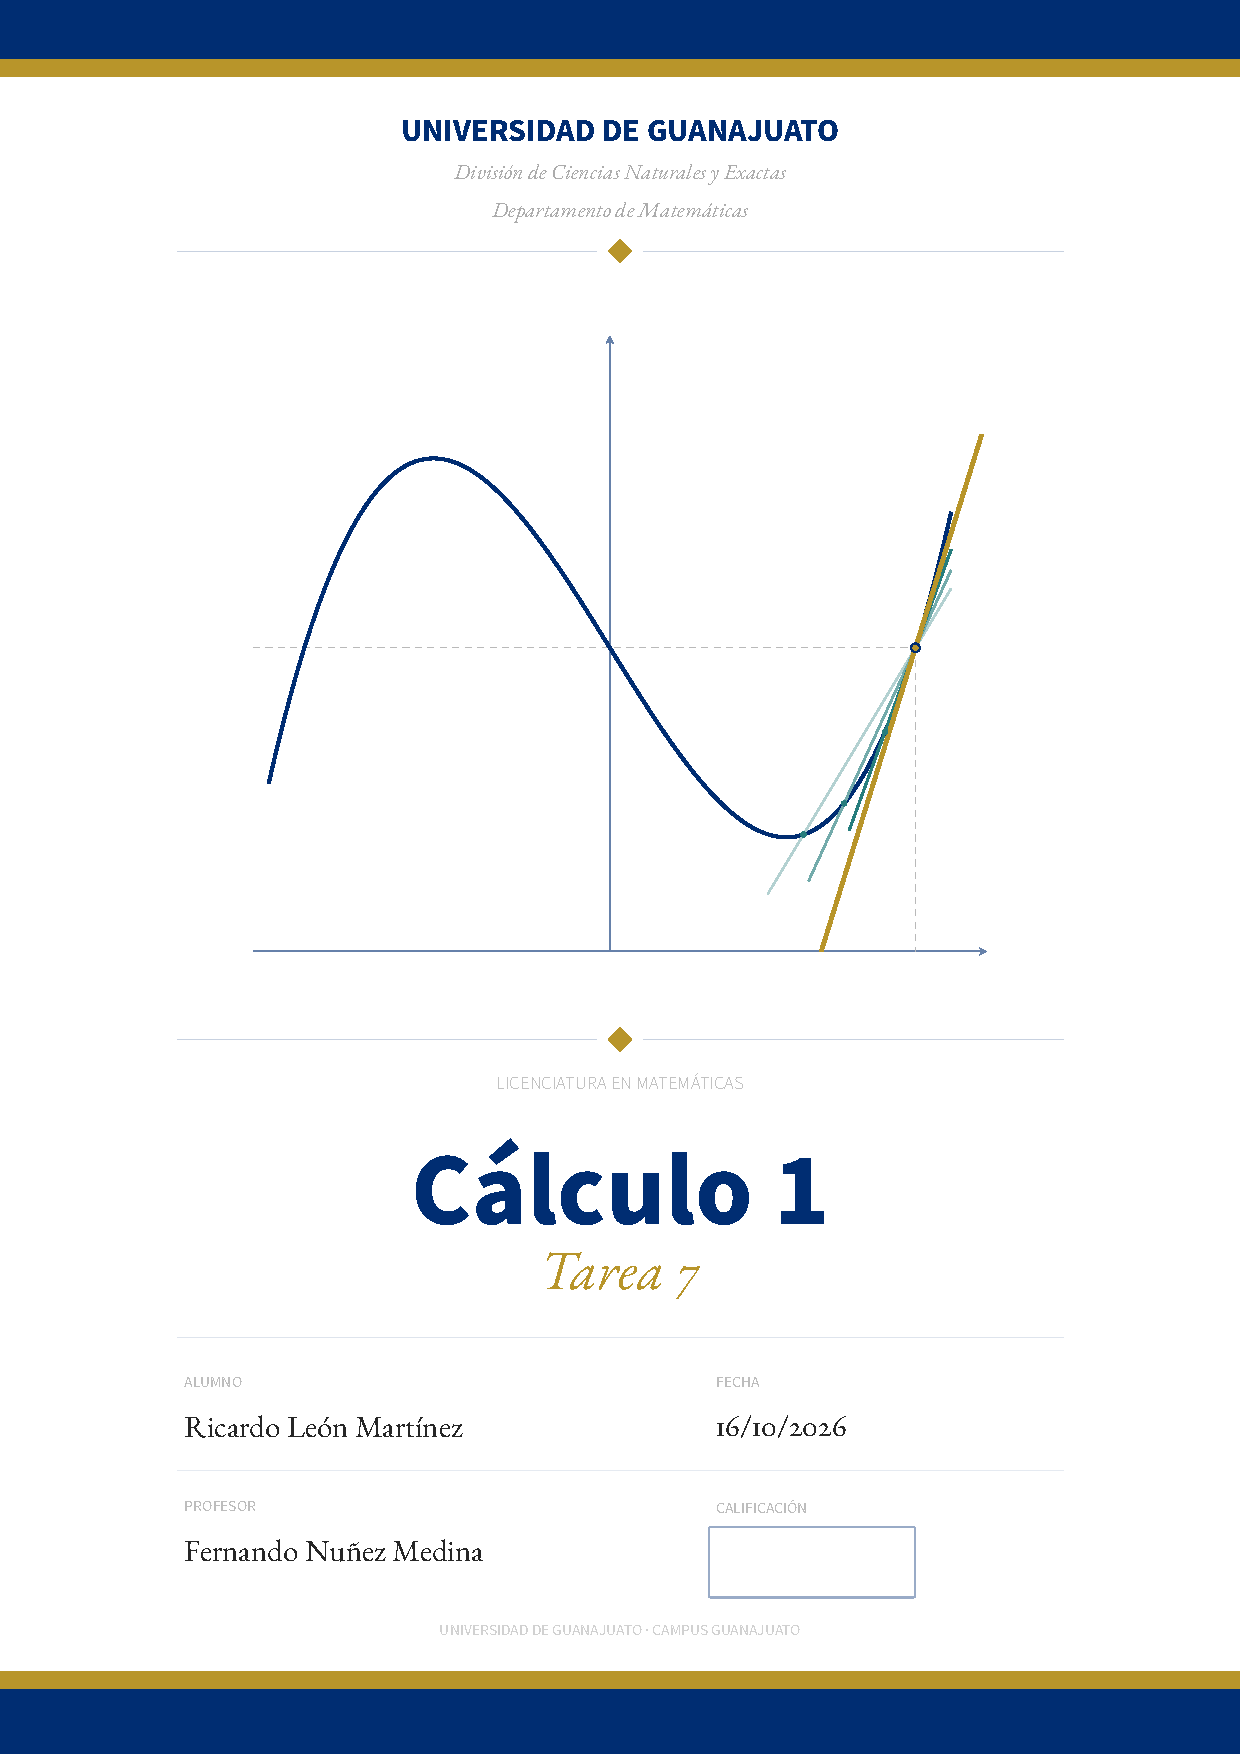
\includepdf[pages=1]{main.pdf}

    \begin{problema}
        \textbf{(Leyes de los exponentes)} Sean $x$ y $y$ números reales, y $m$ y $n$ números naturales tales que las expresiones algebraicas de los incisos siguientes están definidas. Prueba lo siguiente:
        \begin{enumerate}
            \item[(a)] $x^{m}\cdot x^{n}=x^{m+n}.$
            \item[(b)] $\dfrac{x^{m}}{x^{n}}=x^{m-n}.$
            \item[(c)] $x^{n}\cdot y^{n}=(xy)^{n}.$
            \item[(d)] $\left(\dfrac{x}{y}\right)^{n}=\dfrac{x^{n}}{y^{n}}.$
            \item[(e)] $\left(x^{m}\right)^{n}=x^{m\cdot n}.$
        \end{enumerate}
        \textbf{Sugerencia:} Los incisos (a), (c) y (e) son claros. Para probar los incisos (b) y (d), recuerda como se definió la división y ten presente el ejercicio 1 de la tarea 6.
    \end{problema}

    \begin{proof}
        Recordemos que, por la definición 11, $x^{0}=1$, $x^{1}=x$ y, para $n\geq2$, $x^{n}$ es el producto de $x$ consigo mismo $n$ veces. Además, si $x\neq0$, entonces $x^{-n}=\left(x^{n}\right)^{-1}$.

        \textbf{(a)} El número $x^{m}\cdot x^{n}$ es el producto de $m$ factores iguales a $x$ multiplicado por el producto de $n$ factores iguales a $x$. Por la asociatividad del producto y la observación 2 podemos omitir los paréntesis, de modo que $x^{m}\cdot x^{n}$ es el producto de $x$ consigo mismo $m+n$ veces, es decir,
        \begin{equation*}
            x^{m}\cdot x^{n}=x^{m+n}.
        \end{equation*}
        En particular, con $n=1$ obtenemos que para todo $m\in\N$
        \begin{equation*}
            x^{m+1}=x^{m}\cdot x.
        \end{equation*}

        \textbf{(c)} Procederemos por inducción sobre $n$. Si $n=1$, entonces
        \begin{equation*}
            x^{1}\cdot y^{1}=xy=(xy)^{1}.
        \end{equation*}
        Supongamos que $x^{n}\cdot y^{n}=(xy)^{n}$ para algún $n\in\N$. Por el inciso (a), la conmutatividad y asociatividad del producto y la hipótesis de inducción,
        \begin{align*}
            x^{n+1}\cdot y^{n+1}&=\left(x^{n}x\right)\left(y^{n}y\right)\\
            &=\left(x^{n}y^{n}\right)(xy)\\
            &=(xy)^{n}(xy)\\
            &=(xy)^{n+1}.
        \end{align*}
        Por el principio de inducción matemática, que es la proposición 15, la igualdad es válida para todo $n\in\N$.

        \textbf{(e)} Fijemos $m\in\N$ y procedamos por inducción sobre $n$. Si $n=1$, entonces
        \begin{equation*}
            \left(x^{m}\right)^{1}=x^{m}=x^{m\cdot1}.
        \end{equation*}
        Supongamos que $\left(x^{m}\right)^{n}=x^{m\cdot n}$ para algún $n\in\N$. Por el inciso (a), la hipótesis de inducción y la distributividad,
        \begin{equation*}
            \left(x^{m}\right)^{n+1}=\left(x^{m}\right)^{n}x^{m}=x^{m\cdot n}x^{m}=x^{m\cdot n+m}=x^{m\cdot(n+1)}.
        \end{equation*}
        Por el principio de inducción matemática, la igualdad es válida para todo $n\in\N$.

        Sea $x\neq0$. Procederemos por inducción sobre $k$ para ver que $x^{k}\neq0$. Se tiene $x^{1}=x\neq0$. Si $x^{k}\neq0$ para algún $k\in\N$, entonces
        \begin{equation*}
            x^{k+1}=x^{k}x\neq0,
        \end{equation*}
        pues si fuera $x^{k}x=0$, el ejercicio 4 de la tarea 3 daría $x^{k}=0$ o $x=0$, lo cual no es posible. Por el principio de inducción matemática,
        \begin{equation*}
            x^{k}\neq0\quad\text{para todo }k\in\N,
        \end{equation*}
        así que $\left(x^{k}\right)^{-1}$ existe.

        \textbf{(b)} Para que $x^{m}/x^{n}$ esté definido debe ser $x^{n}\neq0$, lo cual obliga a que $x\neq0$, pues si $x=0$, entonces, por la proposición 7, $x^{n}=0$. Por la definición 8 de la división,
        \begin{equation*}
            \frac{x^{m}}{x^{n}}=x^{m}\left(x^{n}\right)^{-1}.
        \end{equation*}
        Distinguimos tres casos.

        \textbf{Caso $m>n$.} Sea $k=m-n\in\N$. Por el inciso (a),
        \begin{equation*}
            x^{m}=x^{n+k}=x^{k}x^{n},
        \end{equation*}
        así que, por la asociatividad del producto y el axioma 8,
        \begin{equation*}
            x^{m}\left(x^{n}\right)^{-1}=x^{k}\left(x^{n}\left(x^{n}\right)^{-1}\right)=x^{k}\cdot1=x^{m-n}.
        \end{equation*}

        \textbf{Caso $m=n$.} Por el axioma 8 y la definición 11,
        \begin{equation*}
            x^{m}\left(x^{n}\right)^{-1}=x^{n}\left(x^{n}\right)^{-1}=1=x^{0}=x^{m-n}.
        \end{equation*}

        \textbf{Caso $m<n$.} Sea $k=n-m\in\N$. Por el inciso (a),
        \begin{equation*}
            x^{n}=x^{m+k}=x^{m}x^{k},
        \end{equation*}
        y como $x^{m}\neq0$ y $x^{k}\neq0$, por el ejercicio 2 de la tarea 4 se tiene
        \begin{equation*}
            \left(x^{n}\right)^{-1}=\left(x^{m}x^{k}\right)^{-1}=\left(x^{m}\right)^{-1}\left(x^{k}\right)^{-1}.
        \end{equation*}
        Así, por la asociatividad del producto, el axioma 8 y la definición 11,
        \begin{equation*}
            x^{m}\left(x^{n}\right)^{-1}=\left(x^{m}\left(x^{m}\right)^{-1}\right)\left(x^{k}\right)^{-1}=\left(x^{k}\right)^{-1}=x^{-k}=x^{m-n}.
        \end{equation*}
        En los tres casos,
        \begin{equation*}
            \frac{x^{m}}{x^{n}}=x^{m-n}.
        \end{equation*}

        \textbf{(d)} Para que $x/y$ esté definido debe ser $y\neq0$, y entonces $y^{n}\neq0$. Por la definición 8 de la división, el inciso (c) y el ejercicio 1 de la tarea 6,
        \begin{equation*}
            \left(\frac{x}{y}\right)^{n}=\left(xy^{-1}\right)^{n}=x^{n}\left(y^{-1}\right)^{n}=x^{n}\left(y^{n}\right)^{-1}=\frac{x^{n}}{y^{n}}.\qedhere
        \end{equation*}
    \end{proof}

    \begin{problema}
        Prueba lo siguiente:
        \begin{enumerate}
            \item[(a)] Si $x>0$, entonces $x^{-1}>0$.
            \item[(b)] Si $x<0$, entonces $x^{-1}<0$.
        \end{enumerate}
        \textbf{Sugerencia:} Procede por contradicción y ten presente el ejercicio 2 de la tarea 6.
    \end{problema}

    \begin{proof}
        En ambos incisos $x\neq0$, así que $x^{-1}$ existe por el axioma 8. Además, $x^{-1}\neq0$, pues si $x^{-1}=0$, entonces, por el axioma 8 y la proposición 7,
        \begin{equation*}
            1=x\cdot x^{-1}=x\cdot0=0,
        \end{equation*}
        lo cual contradice que $1\neq0$ por el axioma 7.

        \textbf{(a)} Procederemos por contradicción. Supongamos que $x>0$ y que no se cumple $x^{-1}>0$. Como $x^{-1}\neq0$, por la tricotomía se tiene $x^{-1}<0$. Como $x>0$ y $x^{-1}<0$, por el inciso (c) de la proposición 10,
        \begin{equation*}
            1=x\cdot x^{-1}<0.
        \end{equation*}
        Pero por el ejercicio 2 de la tarea 6, $1>0$, y por la tricotomía no pueden cumplirse a la vez $1<0$ y $0<1$. Esta contradicción prueba que $x^{-1}>0$.

        \textbf{(b)} Procederemos por contradicción. Supongamos que $x<0$ y que no se cumple $x^{-1}<0$. Como $x^{-1}\neq0$, por la tricotomía se tiene $x^{-1}>0$. Como $x<0$ y $x^{-1}>0$, por el inciso (d) de la proposición 10,
        \begin{equation*}
            1=x\cdot x^{-1}<0,
        \end{equation*}
        lo cual, como en el inciso anterior, contradice que $1>0$. Por lo tanto, $x^{-1}<0$.
    \end{proof}

    \begin{problema}
        Sea $A$ un subconjunto no vacío de números reales.
        \begin{enumerate}
            \item[(a)] Prueba que si $A$ es acotado inferiormente, entonces
            \begin{equation*}
                \sup(-A)=-\inf(A).
            \end{equation*}
            \item[(b)] Prueba que si $A$ es acotado superiormente, entonces
            \begin{equation*}
                \inf(-A)=-\sup(A).
            \end{equation*}
        \end{enumerate}
    \end{problema}

    \begin{proof}
        Aquí $-A=\{-a:a\in A\}$. Sean $u,v\in\R$ con $u\leq v$. Si $u=v$, entonces $-v=-u$, y si $u<v$, sumando $(-u)+(-v)$ a ambos lados y usando la preservación del orden bajo la suma, la conmutatividad y asociatividad de la suma y la propiedad de los inversos aditivos,
        \begin{equation*}
            -v=u+\bigl((-u)+(-v)\bigr)<v+\bigl((-u)+(-v)\bigr)=-u.
        \end{equation*}
        Así, si $u\leq v$, entonces $-v\leq-u$. Además, $-(-a)=a$ para todo $a\in\R$, pues $(-a)+a=0$ y, por la unicidad del inverso aditivo, que es el inciso (a) de la proposición 6, $a$ es el inverso aditivo de $-a$. En particular,
        \begin{equation*}
            -(-A)=\{-(-a):a\in A\}=A.
        \end{equation*}

        \textbf{(a)} Como $A$ es no vacío y acotado inferiormente, por la proposición 12 existe $m=\inf(A)$. Además, $-A$ es no vacío, pues $A$ lo es. Sea $y\in-A$, de modo que $y=-a$ para algún $a\in A$. Como $m$ es cota inferior de $A$, se tiene $m\leq a$, y por lo visto al inicio,
        \begin{equation*}
            y=-a\leq-m.
        \end{equation*}
        Así, $-m$ es cota superior de $-A$. Ahora sea $C$ una cota superior de $-A$. Si $a\in A$, entonces $-a\in-A$, así que $-a\leq C$, y por lo visto al inicio,
        \begin{equation*}
            -C\leq-(-a)=a.
        \end{equation*}
        Como $a\in A$ era arbitrario, $-C$ es cota inferior de $A$, y como $m$ es la máxima cota inferior de $A$, se tiene $-C\leq m$. De nuevo por lo visto al inicio,
        \begin{equation*}
            -m\leq-(-C)=C.
        \end{equation*}
        Por lo tanto, $-m$ es la mínima cota superior de $-A$, y por la definición 15,
        \begin{equation*}
            \sup(-A)=-\inf(A).
        \end{equation*}

        \textbf{(b)} Como $A$ es no vacío y acotado superiormente, por el axioma del supremo existe $s=\sup(A)$. El conjunto $-A$ es no vacío y acotado inferiormente, pues si $a\in A$, entonces $a\leq s$, y por lo visto al inicio,
        \begin{equation*}
            -s\leq-a,
        \end{equation*}
        es decir, $-s$ es cota inferior de $-A$. Aplicando el inciso (a) al conjunto $-A$ y usando que $-(-A)=A$, obtenemos
        \begin{equation*}
            \sup(A)=\sup\bigl(-(-A)\bigr)=-\inf(-A).
        \end{equation*}
        Tomando inversos aditivos en ambos lados y usando que $-(-a)=a$,
        \begin{equation*}
            \inf(-A)=-\sup(A).\qedhere
        \end{equation*}
    \end{proof}

    \begin{problema}
        Sea $n\in\N$. Prueba lo siguiente:
        \begin{enumerate}
            \item[(a)] Si $x<y\leq0$ y $n$ es par, entonces $y^{n}<x^{n}$.
            \item[(b)] Si $0\leq x<y$ y $n$ es par, entonces $x^{n}<y^{n}$.
            \item[(c)] Si $x<y$ y $n$ es impar, entonces $x^{n}<y^{n}$.
        \end{enumerate}
        \textbf{Sugerencia:} Prueba primero que el inciso (b) se cumple en realidad para todo número natural $n$ (usa el principio de inducción matemática) y trata de usar este resultado para probar los incisos (a) y (c).
    \end{problema}

    \begin{proof}
        Sean $0\leq x<y$. Procederemos por inducción sobre $n$. Si $n=1$, entonces $0\leq x^{1}<y^{1}$ es la hipótesis. Supongamos que $0\leq x^{n}<y^{n}$ para algún $n\in\N$. Como $0\leq x^{n}<y^{n}$ y $0\leq x<y$, por el ejercicio 5 de la tarea 3,
        \begin{equation*}
            x^{n+1}=x^{n}x<y^{n}y=y^{n+1}.
        \end{equation*}
        Además,
        \begin{equation*}
            x^{n+1}=x^{n}x\geq0,
        \end{equation*}
        pues si $x^{n}=0$ o $x=0$, entonces $x^{n}x=0$ por la proposición 7, y en otro caso $x^{n}>0$ y $x>0$, así que $x^{n}x>0$ por el inciso (a) de la proposición 10. Por el principio de inducción matemática, que es la proposición 15,
        \begin{equation*}
            0\leq x^{n}<y^{n}\quad\text{para todo }n\in\N\text{ si }0\leq x<y.
        \end{equation*}
        En particular, tomando $x=0$, obtenemos que si $y>0$, entonces $y^{n}>0$ para todo $n\in\N$.

        Por otra parte, para todo $z\in\R$, por las leyes de los signos para la multiplicación, que son el ejercicio 3 de la tarea 3, 
        \begin{equation*}
            (-1)z=-(1\cdot z)=-z\qquad\text{y}\qquad(-1)(-1)=1\cdot1=1.
        \end{equation*}
        Así, por los incisos (c) y (e) de las leyes de los exponentes, que son el ejercicio 1,
        \begin{equation*}
            (-z)^{n}=\bigl((-1)z\bigr)^{n}=(-1)^{n}z^{n}.
        \end{equation*}
        Si $n$ es par, $n=2k$ con $k\in\N$, y
        \begin{equation*}
            (-1)^{n}=\bigl((-1)^{2}\bigr)^{k}=1^{k}=1.
        \end{equation*}
        Si $n$ es impar, entonces $n=1$, en cuyo caso $(-1)^{n}=-1$, o $n=2k+1$ con $k\in\N$, en cuyo caso
        \begin{equation*}
            (-1)^{n}=(-1)^{2k}(-1)=1\cdot(-1)=-1.
        \end{equation*}
        Por lo tanto,
        \begin{equation*}
            (-z)^{n}=z^{n}\quad\text{si }n\text{ es par}\qquad\text{y}\qquad(-z)^{n}=-z^{n}\quad\text{si }n\text{ es impar}.
        \end{equation*}

        \textbf{(b)} Es un caso particular de lo probado por inducción.

        \textbf{(a)} Supongamos que $x<y\leq0$ y que $n$ es par. Por lo visto en el ejercicio 3, de $x<y\leq0$ se sigue
        \begin{equation*}
            0=-0\leq-y<-x,
        \end{equation*}
        así que, por lo probado por inducción, $(-y)^{n}<(-x)^{n}$. Como $n$ es par,
        \begin{equation*}
            y^{n}=(-y)^{n}<(-x)^{n}=x^{n}.
        \end{equation*}

        \textbf{(c)} Supongamos que $x<y$ y que $n$ es impar. Distinguimos tres casos.

        \textbf{Caso $0\leq x$.} Por lo probado por inducción, $x^{n}<y^{n}$.

        \textbf{Caso $x<0\leq y$.} Como $-x>0$, por lo probado por inducción $(-x)^{n}>0$, y como $n$ es impar,
        \begin{equation*}
            x^{n}=-(-x)^{n}<-0=0.
        \end{equation*}
        Por otra parte, si $y=0$, entonces $y^{n}=0$ por la proposición 7, y si $y>0$, entonces $y^{n}>0$ por lo probado por inducción. En ambos casos
        \begin{equation*}
            x^{n}<0\leq y^{n},
        \end{equation*}
        así que $x^{n}<y^{n}$.

        \textbf{Caso $x<y<0$.} Entonces, por el ejercicio 3,
        \begin{equation*}
            0<-y<-x,
        \end{equation*}
        y por lo probado por inducción, $(-y)^{n}<(-x)^{n}$. Como $n$ es impar, esto es
        \begin{equation*}
            -y^{n}<-x^{n},
        \end{equation*}
        y tomando inversos aditivos,
        \begin{equation*}
            x^{n}=-(-x^{n})<-(-y^{n})=y^{n}.
        \end{equation*}
        Como estos casos agotan todas las posibilidades, $x^{n}<y^{n}$.
    \end{proof}

    \begin{problema}
        Sea $f$ una función. Prueba que $f$ es 1-1 ssi $f(A\cap B)=f(A)\cap f(B)$ para todo $A,B\subset\operatorname{dom}(f)$.
    \end{problema}

    \begin{proof}
        Supongamos primero que $f$ es 1-1 y sean $A,B\subset\operatorname{dom}(f)$. Por el inciso (b) del ejercicio 8 de la tarea 4,
        \begin{equation*}
            f(A\cap B)\subset f(A)\cap f(B).
        \end{equation*}
        Sea $y\in f(A)\cap f(B)$. Entonces existen $a\in A$ y $b\in B$ tales que $y=f(a)$ y $y=f(b)$, es decir, $f(a)=f(b)$. Si fuera $a\neq b$, por la definición 25 tendríamos $f(a)\neq f(b)$, lo cual no es así. Por lo tanto, $a=b$. Luego $a\in A\cap B$ y $y=f(a)\in f(A\cap B)$. Así,
        \begin{equation*}
            f(A)\cap f(B)\subset f(A\cap B),
        \end{equation*}
        y por lo tanto,
        \begin{equation*}
            f(A\cap B)=f(A)\cap f(B).
        \end{equation*}

        Recíprocamente, procederemos por contradicción. Supongamos que $f(A\cap B)=f(A)\cap f(B)$ para todo $A,B\subset\operatorname{dom}(f)$ y que $f$ no es 1-1. Entonces existen $x,y\in\operatorname{dom}(f)$ con $x\neq y$ y $f(x)=f(y)$. Tomemos $A=\{x\}$ y $B=\{y\}$. Como $x\neq y$, se tiene $A\cap B=\varnothing$, así que
        \begin{equation*}
            f(A\cap B)=f(\varnothing)=\varnothing.
        \end{equation*}
        Por otra parte,
        \begin{equation*}
            f(A)\cap f(B)=\{f(x)\}\cap\{f(y)\}=\{f(x)\}\neq\varnothing,
        \end{equation*}
        lo cual contradice que $f(A\cap B)=f(A)\cap f(B)$. Por lo tanto, $f$ es 1-1.
    \end{proof}

    \begin{problema}
        Prueba que para todo par de números $x$ y $y$ se cumple lo siguiente:
        \begin{multicols}{2}
            \begin{enumerate}
                \item[(a)] $|x-y|\leq|x|+|y|.$
                \item[(b)] $|x|-|y|\leq|x-y|.$
                \item[(c)] $\bigl||x|-|y|\bigr|\leq|x-y|.$
            \end{enumerate}
        \end{multicols}
        \textbf{Sugerencia:} Trata de usar la desigualdad del triángulo.
    \end{problema}

    \begin{proof}
        Por el ejercicio 2 de la tarea 6, $1>0$, así que, sumando $-1$ a ambos lados, $-1<0$, y por la definición 19,
        \begin{equation*}
            |-1|=-(-1)=1.
        \end{equation*}
        Si $z\in\R$, como $-z=(-1)z$ por las leyes de los signos para la multiplicación, que son el ejercicio 3 de la tarea 3, el inciso (b) de la proposición 31 da
        \begin{equation*}
            |-z|=|(-1)z|=|-1||z|=|z|.
        \end{equation*}
        En particular,
        \begin{equation*}
            |y-x|=|-(x-y)|=|x-y|.
        \end{equation*}

        \textbf{(a)} Por la definición 8 de la resta, la desigualdad del triángulo, que es el inciso (a) de la proposición 31, y lo anterior,
        \begin{equation*}
            |x-y|=|x+(-y)|\leq|x|+|-y|=|x|+|y|.
        \end{equation*}

        \textbf{(b)} Como $x=(x-y)+y$, por la desigualdad del triángulo,
        \begin{equation*}
            |x|=|(x-y)+y|\leq|x-y|+|y|.
        \end{equation*}
        Sumando $-|y|$ a ambos lados y usando la preservación del orden bajo la suma obtenemos
        \begin{equation*}
            |x|-|y|\leq|x-y|.
        \end{equation*}

        \textbf{(c)} Por el inciso (b) aplicado a $x$ y $y$, y luego aplicado a $y$ y $x$,
        \begin{equation*}
            |x|-|y|\leq|x-y|\qquad\text{y}\qquad|y|-|x|\leq|y-x|=|x-y|.
        \end{equation*}
        Tomando inversos aditivos en la segunda desigualdad y usando lo visto en el ejercicio 3 obtenemos
        \begin{equation*}
            -|x-y|\leq|x|-|y|,
        \end{equation*}
        así que
        \begin{equation*}
            -|x-y|\leq|x|-|y|\leq|x-y|.
        \end{equation*}
        Si $|x-y|>0$, el inciso (a) del corolario 1 con $r=|x-y|$ da la desigualdad buscada. Si $|x-y|=0$, por el inciso (b) de la proposición 30 se tiene $x-y=0$, es decir, $x=y$, y entonces
        \begin{equation*}
            \bigl||x|-|y|\bigr|=|0|=0=|x-y|.
        \end{equation*}
        En ambos casos,
        \begin{equation*}
            \bigl||x|-|y|\bigr|\leq|x-y|.\qedhere
        \end{equation*}
    \end{proof}

    \begin{problema}
        Calcula los límites siguientes:
        \begin{multicols}{2}
            \begin{enumerate}
                \item[(a)] $\displaystyle\lim_{x\to8}(x+2)\sqrt[3]{x}.$
                \item[(b)] $\displaystyle\lim_{x\to-1}\frac{x^{2}+4x+3}{x+1}.$
                \item[(c)] $\displaystyle\lim_{x\to-5}\ln(x+6).$
                \item[(d)] $\displaystyle\lim_{x\to1^{+}}\left(2x^{3}-x+5\right).$
                \item[(e)] $\displaystyle\lim_{x\to-\infty}e^{x}\arctan(x).$
                \item[(f)] $\displaystyle\lim_{x\to\infty}\frac{5x^{4}-4x^{2}}{3x^{4}+2x}.$
                \item[(g)] $\displaystyle\lim_{x\to\frac{\pi}{2}^{-}}\left(\sin(x)+\cos(x)+\frac{\sin(x)}{\cos(x)}\right).$
                \item[(h)] $\displaystyle\lim_{x\to\infty}\left(3x^{3}-2x^{2}+x-4\right).$
            \end{enumerate}
        \end{multicols}
    \end{problema}

    \begin{solucion}
        \begin{enumerate}
            \item[(a)] Por el ejemplo 48 del límite de un polinomio y por el inciso (d) de la proposición 33 con $n=3$, que es impar,
            \begin{equation*}
                \lim_{x\to8}(x+2)=8+2=10\qquad\text{y}\qquad\lim_{x\to8}\sqrt[3]{x}=\sqrt[3]{8}=2.
            \end{equation*}
            Así, por el inciso (c) del álgebra de límites de la proposición 36,
            \begin{equation*}
                \lim_{x\to8}(x+2)\sqrt[3]{x}=\lim_{x\to8}(x+2)\cdot\lim_{x\to8}\sqrt[3]{x}=10\cdot2=20.
            \end{equation*}
            \item[(b)] No podemos usar el inciso (d) del álgebra de límites de la proposición 36, pues el límite del denominador es $0$. Factorizando el numerador,
            \begin{equation*}
                x^{2}+4x+3=(x+1)(x+3),
            \end{equation*}
            de modo que, para $x\neq-1$,
            \begin{equation*}
                \frac{x^{2}+4x+3}{x+1}=x+3.
            \end{equation*}
            Por la proposición 37 y el ejemplo 48 del límite de un polinomio,
            \begin{equation*}
                \lim_{x\to-1}\frac{x^{2}+4x+3}{x+1}=\lim_{x\to-1}(x+3)=-1+3=2.
            \end{equation*}
            \item[(c)] Sea $g(x)=x+6$, definida en $I=(-6,-4)$, que contiene a $-5$. Por el ejemplo 48 del límite de un polinomio,
            \begin{equation*}
                \lim_{x\to-5}g(x)=-5+6=1.
            \end{equation*}
            Además, $g(I)=(0,2)\subset(0,\infty)$, que es un intervalo abierto que contiene a $1$ en el que está definido $\ln$, y por el inciso (a) de la proposición 35,
            \begin{equation*}
                \lim_{x\to1}\ln(x)=\ln(1)=0.
            \end{equation*}
            Así, por la proposición 41 del límite de una función compuesta,
            \begin{equation*}
                \lim_{x\to-5}\ln(x+6)=\ln(1)=0.
            \end{equation*}
            \item[(d)] Por el ejemplo 48 del límite de un polinomio,
            \begin{equation*}
                \lim_{x\to1}\left(2x^{3}-x+5\right)=2(1)^{3}-1+5=6.
            \end{equation*}
            Luego, por la proposición 42, que es el criterio de los límites laterales,
            \begin{equation*}
                \lim_{x\to1^{+}}\left(2x^{3}-x+5\right)=6.
            \end{equation*}
            \item[(e)] Por los incisos (g) y (f) de la proposición 44 de límites al infinito básicos,
            \begin{equation*}
                \lim_{x\to-\infty}e^{x}=0\qquad\text{y}\qquad\lim_{x\to-\infty}\arctan(x)=-\frac{\pi}{2}.
            \end{equation*}
            Así, por el álgebra de límites al infinito de la observación 13,
            \begin{equation*}
                \lim_{x\to-\infty}e^{x}\arctan(x)=\lim_{x\to-\infty}e^{x}\cdot\lim_{x\to-\infty}\arctan(x)=0\cdot\left(-\frac{\pi}{2}\right)=0.
            \end{equation*}
            \item[(f)] La función es racional, con numerador y denominador de grado $4$ y coeficientes principales $5$ y $3$, respectivamente. Como los grados son iguales, por el inciso (b) de la proposición 45 de límites al infinito de funciones racionales,
            \begin{equation*}
                \lim_{x\to\infty}\frac{5x^{4}-4x^{2}}{3x^{4}+2x}=\frac{5}{3}.
            \end{equation*}
            \item[(g)] Por los incisos (a) y (b) de la proposición 34 y el criterio de los límites laterales, que es la proposición 42,
            \begin{equation*}
                \lim_{x\to\frac{\pi}{2}^{-}}\sin(x)=\sin\left(\frac{\pi}{2}\right)=1\qquad\text{y}\qquad\lim_{x\to\frac{\pi}{2}^{-}}\cos(x)=\cos\left(\frac{\pi}{2}\right)=0.
            \end{equation*}
            Además, $\frac{\sin(x)}{\cos(x)}=\tan(x)$, y por el inciso (g) de la proposición 47 de límites infinitos básicos,
            \begin{equation*}
                \lim_{x\to\frac{\pi}{2}^{-}}\tan(x)=\infty.
            \end{equation*}
            Así, por el álgebra de límites laterales infinitos de la observación 16,
            \begin{equation*}
                \lim_{x\to\frac{\pi}{2}^{-}}\left(\sin(x)+\cos(x)+\frac{\sin(x)}{\cos(x)}\right)=1+0+\infty=\infty.
            \end{equation*}
            Es decir, el límite existe como límite infinito, pero no existe como límite real.
            \item[(h)] El polinomio $3x^{3}-2x^{2}+x-4$ es no constante y su coeficiente principal es $3>0$. Por la proposición 52 de límites infinitos al infinito de un polinomio no constante,
            \begin{equation*}
                \lim_{x\to\infty}\left(3x^{3}-2x^{2}+x-4\right)=\lim_{x\to\infty}3x^{3}=\infty.
            \end{equation*}
            Es decir, el límite existe como límite infinito al infinito, pero no existe como límite al infinito.
        \end{enumerate}
    \end{solucion}

    \begin{problema}
        Prueba que $\displaystyle\lim_{x\to p}f(x)=L$ ssi $\displaystyle\lim_{x\to p}\bigl(f(x)-L\bigr)=0$.
    \end{problema}

    \begin{proof}
        Sea $I$ un intervalo abierto que contiene a $p$ en el que $f$ está definida, excepto posiblemente en $p$. La función $g(x)=f(x)-L$ está definida exactamente donde lo está $f$, así que también está definida en $I$, excepto posiblemente en $p$. Además, para todo $x\in I\setminus\{p\}$,
        \begin{equation*}
            |g(x)-0|=|f(x)-L|.
        \end{equation*}

        Supongamos primero que $\lim_{x\to p}f(x)=L$ y sea $\e>0$. Por la definición 28, existe $\delta>0$ tal que si $x\in I$ y $0<|x-p|<\delta$, entonces $|f(x)-L|<\e$. Luego, si $x\in I$ y $0<|x-p|<\delta$, entonces
        \begin{equation*}
            |g(x)-0|=|f(x)-L|<\e.
        \end{equation*}
        Como $\e>0$ era arbitrario,
        \begin{equation*}
            \lim_{x\to p}\bigl(f(x)-L\bigr)=0.
        \end{equation*}

        Recíprocamente, supongamos que $\lim_{x\to p}\bigl(f(x)-L\bigr)=0$ y sea $\e>0$. Por la definición 28, existe $\delta>0$ tal que si $x\in I$ y $0<|x-p|<\delta$, entonces $|g(x)-0|<\e$. Luego, si $x\in I$ y $0<|x-p|<\delta$, entonces
        \begin{equation*}
            |f(x)-L|=|g(x)-0|<\e.
        \end{equation*}
        Como $\e>0$ era arbitrario,
        \begin{equation*}
            \lim_{x\to p}f(x)=L.\qedhere
        \end{equation*}
    \end{proof}

    \begin{problema}
        Prueba que $\displaystyle\lim_{x\to p}f(x)=0$ ssi $\displaystyle\lim_{x\to p}|f(x)|=0$.
    \end{problema}

    \begin{proof}
        Sea $I$ un intervalo abierto que contiene a $p$ en el que $f$ está definida, excepto posiblemente en $p$. La función $|f(x)|$ está definida en el mismo conjunto. Para todo $x\in I\setminus\{p\}$, por el inciso (a) de la proposición 30 se tiene $|f(x)|\geq0$, y por la definición 19 del valor absoluto,
        \begin{equation*}
            \bigl||f(x)|-0\bigr|=\bigl||f(x)|\bigr|=|f(x)|=|f(x)-0|.
        \end{equation*}

        Supongamos primero que $\lim_{x\to p}f(x)=0$ y sea $\e>0$. Por la definición 28, existe $\delta>0$ tal que si $x\in I$ y $0<|x-p|<\delta$, entonces $|f(x)-0|<\e$. Luego, si $x\in I$ y $0<|x-p|<\delta$, entonces
        \begin{equation*}
            \bigl||f(x)|-0\bigr|=|f(x)-0|<\e.
        \end{equation*}
        Como $\e>0$ era arbitrario,
        \begin{equation*}
            \lim_{x\to p}|f(x)|=0.
        \end{equation*}

        Recíprocamente, supongamos que $\lim_{x\to p}|f(x)|=0$ y sea $\e>0$. Por la definición 28, existe $\delta>0$ tal que si $x\in I$ y $0<|x-p|<\delta$, entonces $\bigl||f(x)|-0\bigr|<\e$. Luego, si $x\in I$ y $0<|x-p|<\delta$, entonces
        \begin{equation*}
            |f(x)-0|=\bigl||f(x)|-0\bigr|<\e.
        \end{equation*}
        Como $\e>0$ era arbitrario,
        \begin{equation*}
            \lim_{x\to p}f(x)=0.\qedhere
        \end{equation*}
    \end{proof}

    \begin{problema}
        Prueba que $\displaystyle\lim_{x\to p}f(x)=L$ ssi $\displaystyle\lim_{h\to0}f(p+h)=L$.
    \end{problema}

    \begin{proof}
        Sea $I$ un intervalo abierto que contiene a $p$ en el que $f$ está definida, excepto posiblemente en $p$, y definamos
        \begin{equation*}
            g(h)=f(p+h)\qquad\text{y}\qquad J=\{h:p+h\in I\}.
        \end{equation*}
        Como $J=\{x-p:x\in I\}$ e $I$ es un intervalo abierto que contiene a $p$, $J$ es un intervalo abierto que contiene a $0$, y $g$ está definida en $J$, excepto posiblemente en $0$, pues $p+h\neq p$ si $h\neq0$.

        Supongamos primero que $\lim_{x\to p}f(x)=L$ y sea $\e>0$. Por la definición 28, existe $\delta>0$ tal que si $x\in I$ y $0<|x-p|<\delta$, entonces $|f(x)-L|<\e$. Sea $h\in J$ con $0<|h-0|<\delta$ y tomemos $x=p+h$. Entonces $x\in I$ y $0<|x-p|=|h|<\delta$, así que
        \begin{equation*}
            |g(h)-L|=|f(p+h)-L|=|f(x)-L|<\e.
        \end{equation*}
        Como $\e>0$ era arbitrario,
        \begin{equation*}
            \lim_{h\to0}f(p+h)=L.
        \end{equation*}

        Recíprocamente, supongamos que $\lim_{h\to0}f(p+h)=L$ y sea $\e>0$. Por la definición 28, existe $\delta>0$ tal que si $h\in J$ y $0<|h-0|<\delta$, entonces $|f(p+h)-L|<\e$. Sea $x\in I$ con $0<|x-p|<\delta$ y tomemos $h=x-p$. Entonces $p+h=x\in I$, es decir, $h\in J$, y $0<|h-0|=|x-p|<\delta$, así que
        \begin{equation*}
            |f(x)-L|=|f(p+h)-L|<\e.
        \end{equation*}
        Como $\e>0$ era arbitrario,
        \begin{equation*}
            \lim_{x\to p}f(x)=L.\qedhere
        \end{equation*}
    \end{proof}

\end{document}
